\documentclass[10pt]{beamer}

\usepackage[utf8]{inputenc}
\usepackage[french]{babel}
\usepackage{amsfonts,amsmath,amssymb,bbold,dsfont}
\usepackage{calrsfs}
\usepackage[lined,boxed, ruled,vlined, french]{algorithm2e}
\usepackage{multirow}
\usepackage{mathtools,mathptmx}
\usepackage{empheq}
\usepackage{enumerate}
\usepackage{makecell}
\usepackage{tabularx}
%% for images print :
\usepackage{svg}
\usepackage{tikz}
\usetikzlibrary{tikzmark,calc,arrows,shapes,decorations.pathreplacing}
\tikzset{every picture/.style={remember picture}}
\usepackage{accents}
\newcommand\myubar[1]{\underaccent{\bar}{#1}}
\usepackage{comment}
\usepackage{natbib}

%%% theme of diapo %%%%%%%%%%%%%%%%%%%%%%%%%%%%%%%%%%%%%%%%%%%%%%%%%%%%%%%%%%%
%\usetheme{PaloAlto}
\usecolortheme{seahorse}

%%%%title page
\defbeamertemplate*{title page}{customized}[1][]
{
    \begin{center}
    \usebeamerfont{title}\inserttitle\par
  %\usebeamerfont{subtitle}\usebeamercolor[fg]{subtitle}\insertsubtitle\par
    \vfill
      \begin{minipage}{0.3\textwidth}
        \begin{center} 
            
\includegraphics[width=.8\linewidth]{logo_LBBE.png}
        \end{center}
    \end{minipage}
    \begin{minipage}{0.3\textwidth}
        \hfill
    \end{minipage}
    \begin{minipage}{0.3\textwidth}
        \begin{center} 
            
\includegraphics[width=.8\linewidth]{logo_UCBL.png}
        \end{center}
    \end{minipage}
    \vfill
    \insertauthor\par
    \insertdate\par
   \end{center}
  }
%%%%% footer
\defbeamertemplate*{footline}{my footline}{
	\leavevmode%
	\hbox{%
		\begin{beamercolorbox}[wd=.3\paperwidth,ht=2.25ex,dp=1ex,center]{author in head/foot}%
			\usebeamerfont{author in head/foot}\insertshortauthor
		\end{beamercolorbox}%
		\begin{beamercolorbox}[wd=.6\paperwidth,ht=2.25ex,dp=1ex,center]{title in head/foot}%
			\usebeamerfont{title in head/foot}\insertshorttitle
		\end{beamercolorbox}%
		\begin{beamercolorbox}[wd=.1\paperwidth,ht=2.25ex,dp=1ex,center]{date in head/foot}%
			\insertframenumber{} / \inserttotalframenumber\hspace*{1ex}
	\end{beamercolorbox}}%
	\vskip 0pt%
    }
%\beamertemplatenavigationsymbolsempty





%%%%%%%%%%%%%%%%%%%%%%%%%%%%%%%%%%%%%%%%%%%%%%%%%%%%%%%%%%%%%%%%%%%%%%%%%%%%

\title{"Kernel V0" \\ Définition et premières propriétés}
\author{Antoine Villié et Claire Gayral}
%\institute{Université Claude Bernard, Lyon 1}
\date{9 Janvier 2020}
%\bibliography{<pres_biblio>}

%%%%%%%%%%%%%%%%%%%%%%%%%%%%%%%%%%%%%%%%%%%%%%%%%%%%%%%%%%%%%%%%%%%%%%%%%%%%%

\begin{document}
\begin{frame}{}
    \frametitle{}
    %{\huge } 
    \titlepage
\end{frame}

\begin{frame}{Kernel : definition}
    \begin{center} 
        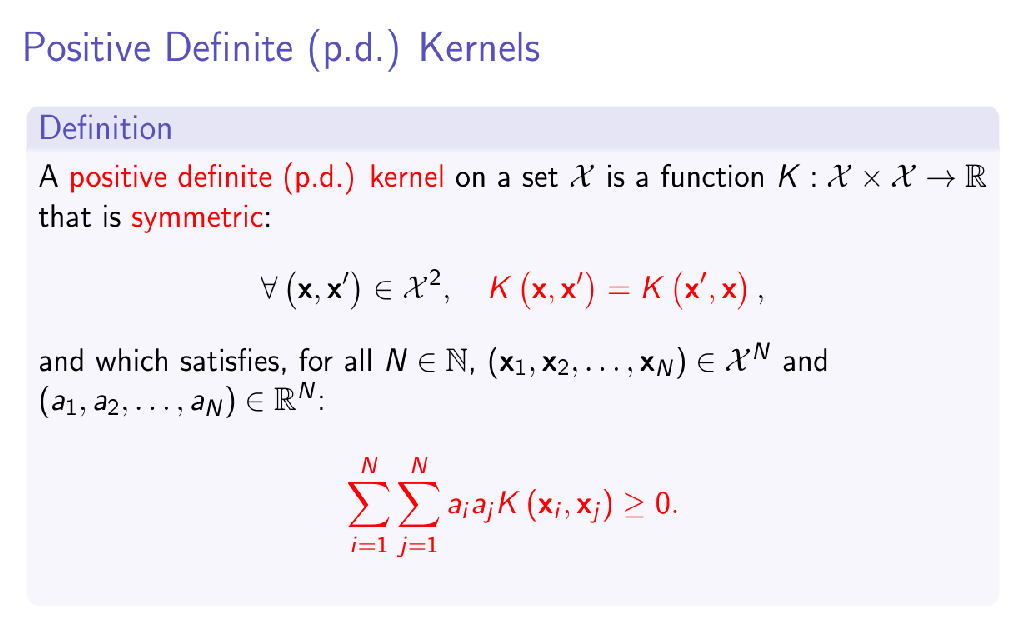
\includegraphics[width=.99\linewidth]{JPV_slide14.png}
    \end{center}
    from J.P. Vert and J. Mairal slides
\end{frame}

\begin{frame}{First Example : Polynomial Kernel}
    \begin{overprint}
    \onslide<1->
    \begin{center} 
        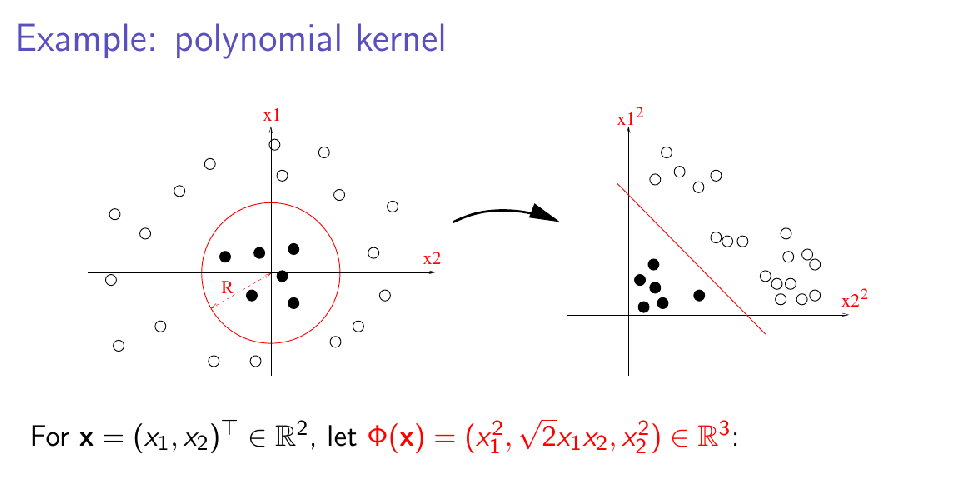
\includegraphics[width=.99\linewidth]{JPV_slide19.png}
    \end{center}
    
    \onslide<2->
    \begin{center} 
        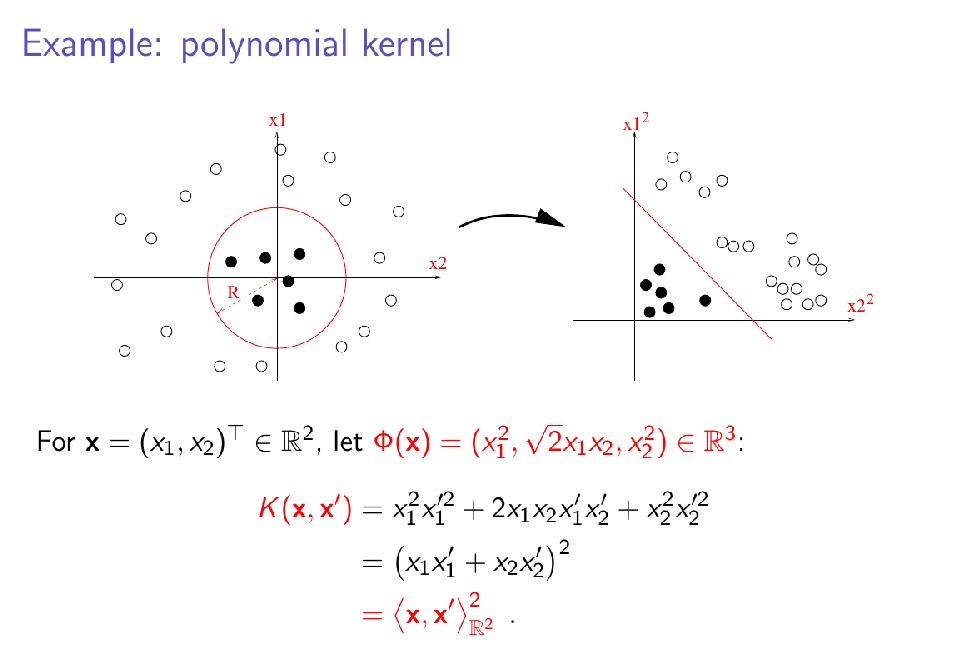
\includegraphics[width=.99\linewidth]{JPV_slide19b.png}
    \end{center}
    \end{overprint}
    from J.P. Vert and J. Mairal slides
\end{frame}

\begin{frame}{Aronszajn Theorem}
    \begin{center} 
        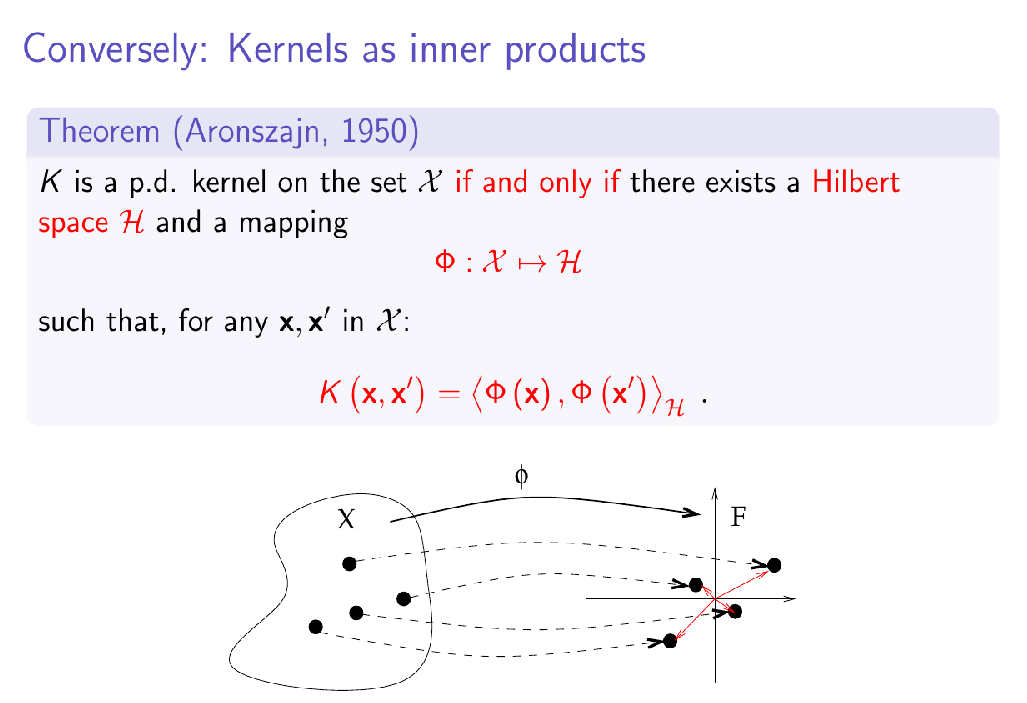
\includegraphics[width=.99\linewidth]{kernel_sgdg2020/JPV_slide20.png}
    \end{center}
    from J.P. Vert and J. Mairal slides
\end{frame}

\begin{frame}{Some properties}
    \begin{center} 
        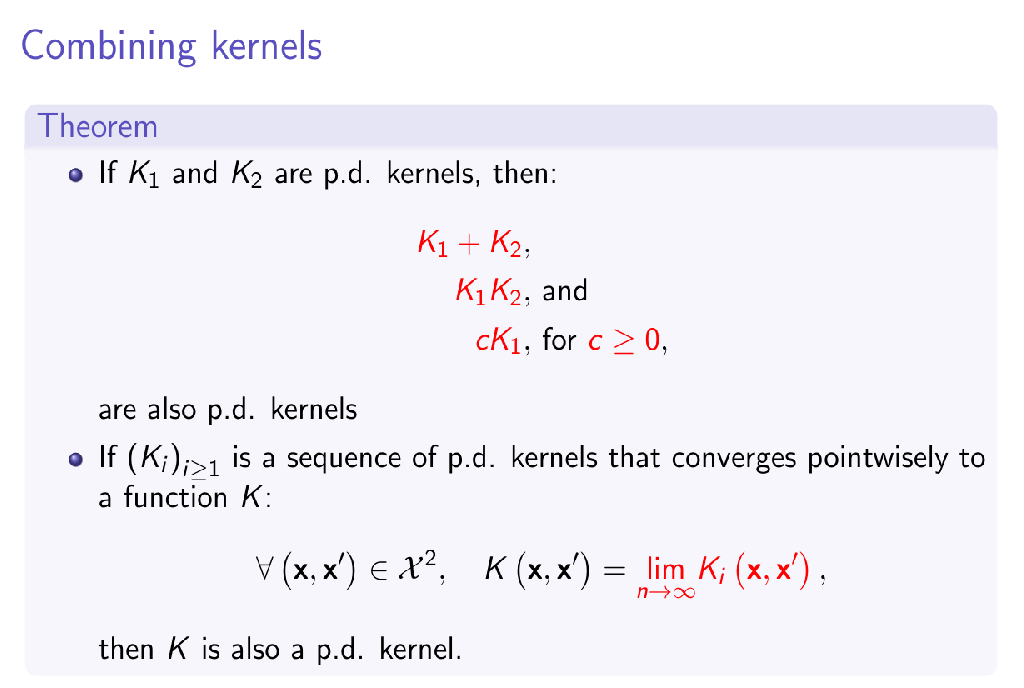
\includegraphics[width=.99\linewidth]{kernel_sgdg2020/JPV_slide47.png}
    \end{center}
    from J.P. Vert and J. Mairal slides
\end{frame}

\begin{frame}{Some properties}
    \begin{center} 
        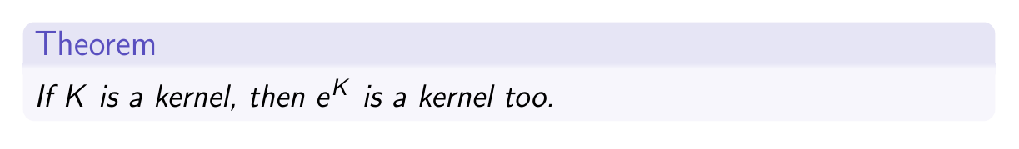
\includegraphics[width=.99\linewidth]{kernel_sgdg2020/JPV_slide49.png}
    \end{center}
    from J.P. Vert and J. Mairal slides
\end{frame}

\end{document}
